\documentclass{beamer}
\input{../style/cours-style.sty}

% Title
\title[PYTHON]{Introduction à la programmation Python}
\author{Christophe Brun}
\institute{Digicomp}
\date{17 mai 2024}
\beamertemplatenavigationsymbolsempty

\titlegraphic{
    \bigbreak
    
\includegraphics[width=5cm]{image/digicomp-logo}
    \bigbreak
    Digital competence. Made of People.
    \bigbreak
}

\begin{document}

    \begin{frame}
        \titlepage
        \bigbreak
        \centering
        \url{https://github.com/DigicompClassesByPapIT/Python}
    \end{frame}


    \section{Table des matières}\label{sec:toc}

    \begin{frame}{Table des matières}
        \begin{tiny}
            \begin{multicols}{2}
                \tableofcontents
            \end{multicols}
        \end{tiny}
    \end{frame}


    \section{Programme du module}\label{sec:programme-du-module}

    \begin{frame}{Introduction à la programmation Python}{Contenu des 3 jours}
            \begin{multicols}{3}
                \begin{tiny}
                    \begin{enumerate}
                        \item Qu'est-ce que Python ?
                        \item Premiers pas
                        \begin{itemize}
                            \begin{tiny}
                                \item Opérations arithmétiques
                                \item Premier programme
                                \item Enregistrer et exécuter
                            \end{tiny}
                        \end{itemize}

                        \item Bases de la programmation
                        \begin{itemize}
                            \begin{tiny}
                                \item Variables et opérateurs
                                \item Branchements
                                \item Boucles
                                \item Erreurs et exceptions
                                \item Fonctions
                            \end{tiny}
                        \end{itemize}

                        \item Types de données
                        \begin{itemize}
                            \begin{tiny}
                                \item Nombres
                                \item Strings
                                \item Listes
                                \item Dictionnaires
                                \item Ensembles (Sets)
                            \end{tiny}
                        \end{itemize}

                        \item Programmation avancée
                        \begin{itemize}
                            \begin{tiny}
                                \item Sortie et mise en forme
                                \item Erreurs et exceptions
                                \item Fonctions
                                \item Modules propres
                                \item Les paramètres de la ligne de commande
                            \end{tiny}
                        \end{itemize}

                        \item Différents modules
                        \begin{itemize}
                            \begin{tiny}
                                \item Date et heure
                                \item Expressions régulières
                                \item Charger des nouveaux modules
                            \end{tiny}
                        \end{itemize}

                        \item Fichiers
                        \begin{itemize}
                            \begin{tiny}
                                \item Décrire des fichiers
                                \item Lecture des fichiers
                            \end{tiny}
                        \end{itemize}

                        \item Internet
                        \begin{itemize}
                            \begin{tiny}
                                \item Lire des pages web
                                \item Copier des pages web
                                \item Envoyer des données avec GET et POST
                            \end{tiny}
                        \end{itemize}

                        \item Bases de données
                        \begin{itemize}
                            \begin{tiny}
                                \item Créer des bases de données, tables
                                \item Lire des données
                                \item Sélectionnez des données
                                \item Changement des données
                                \item Effacer des données
                            \end{tiny}
                        \end{itemize}

                        \item Interfaces utilisateurs
                        \begin{itemize}
                            \begin{tiny}
                                \item Introduction à la programmation d'interfaces graphiques

                            \end{tiny}
                        \end{itemize}

                        \item Programmation avec l'intelligence artificielle
                    \end{enumerate}
                \end{tiny}
            \end{multicols}
    \end{frame}


    \section{Introduction}\label{sec:introduction}

    \begin{frame}{Formateur sur Linux}{Christophe Brun, conseil en développement informatique}

        \begin{columns}
            \column{0.7\textwidth}
            \begin{itemize}
                \item Développeur freelance (Python, Java, CoBOL) et data at scale.

                \item 7 ans de conseil en développement au sein d'SSII~.

                \item 7 ans de conseil en développement en indépendant, \href{https://papit.fr}{PapIT}.

                \item Passionné~!
                \bigbreak
                \begin{columns}
                    \column{0.5\textwidth}
                    \centering
                    
\includegraphics[width=3cm]{image/logo-uppa}
                    \column{0.5\textwidth}
                    \centering
                    
\includegraphics[width=3cm]{image/logo-universite-bordeaux}
                \end{columns}
            \end{itemize}
            \column{0.3\textwidth}
            \centering
            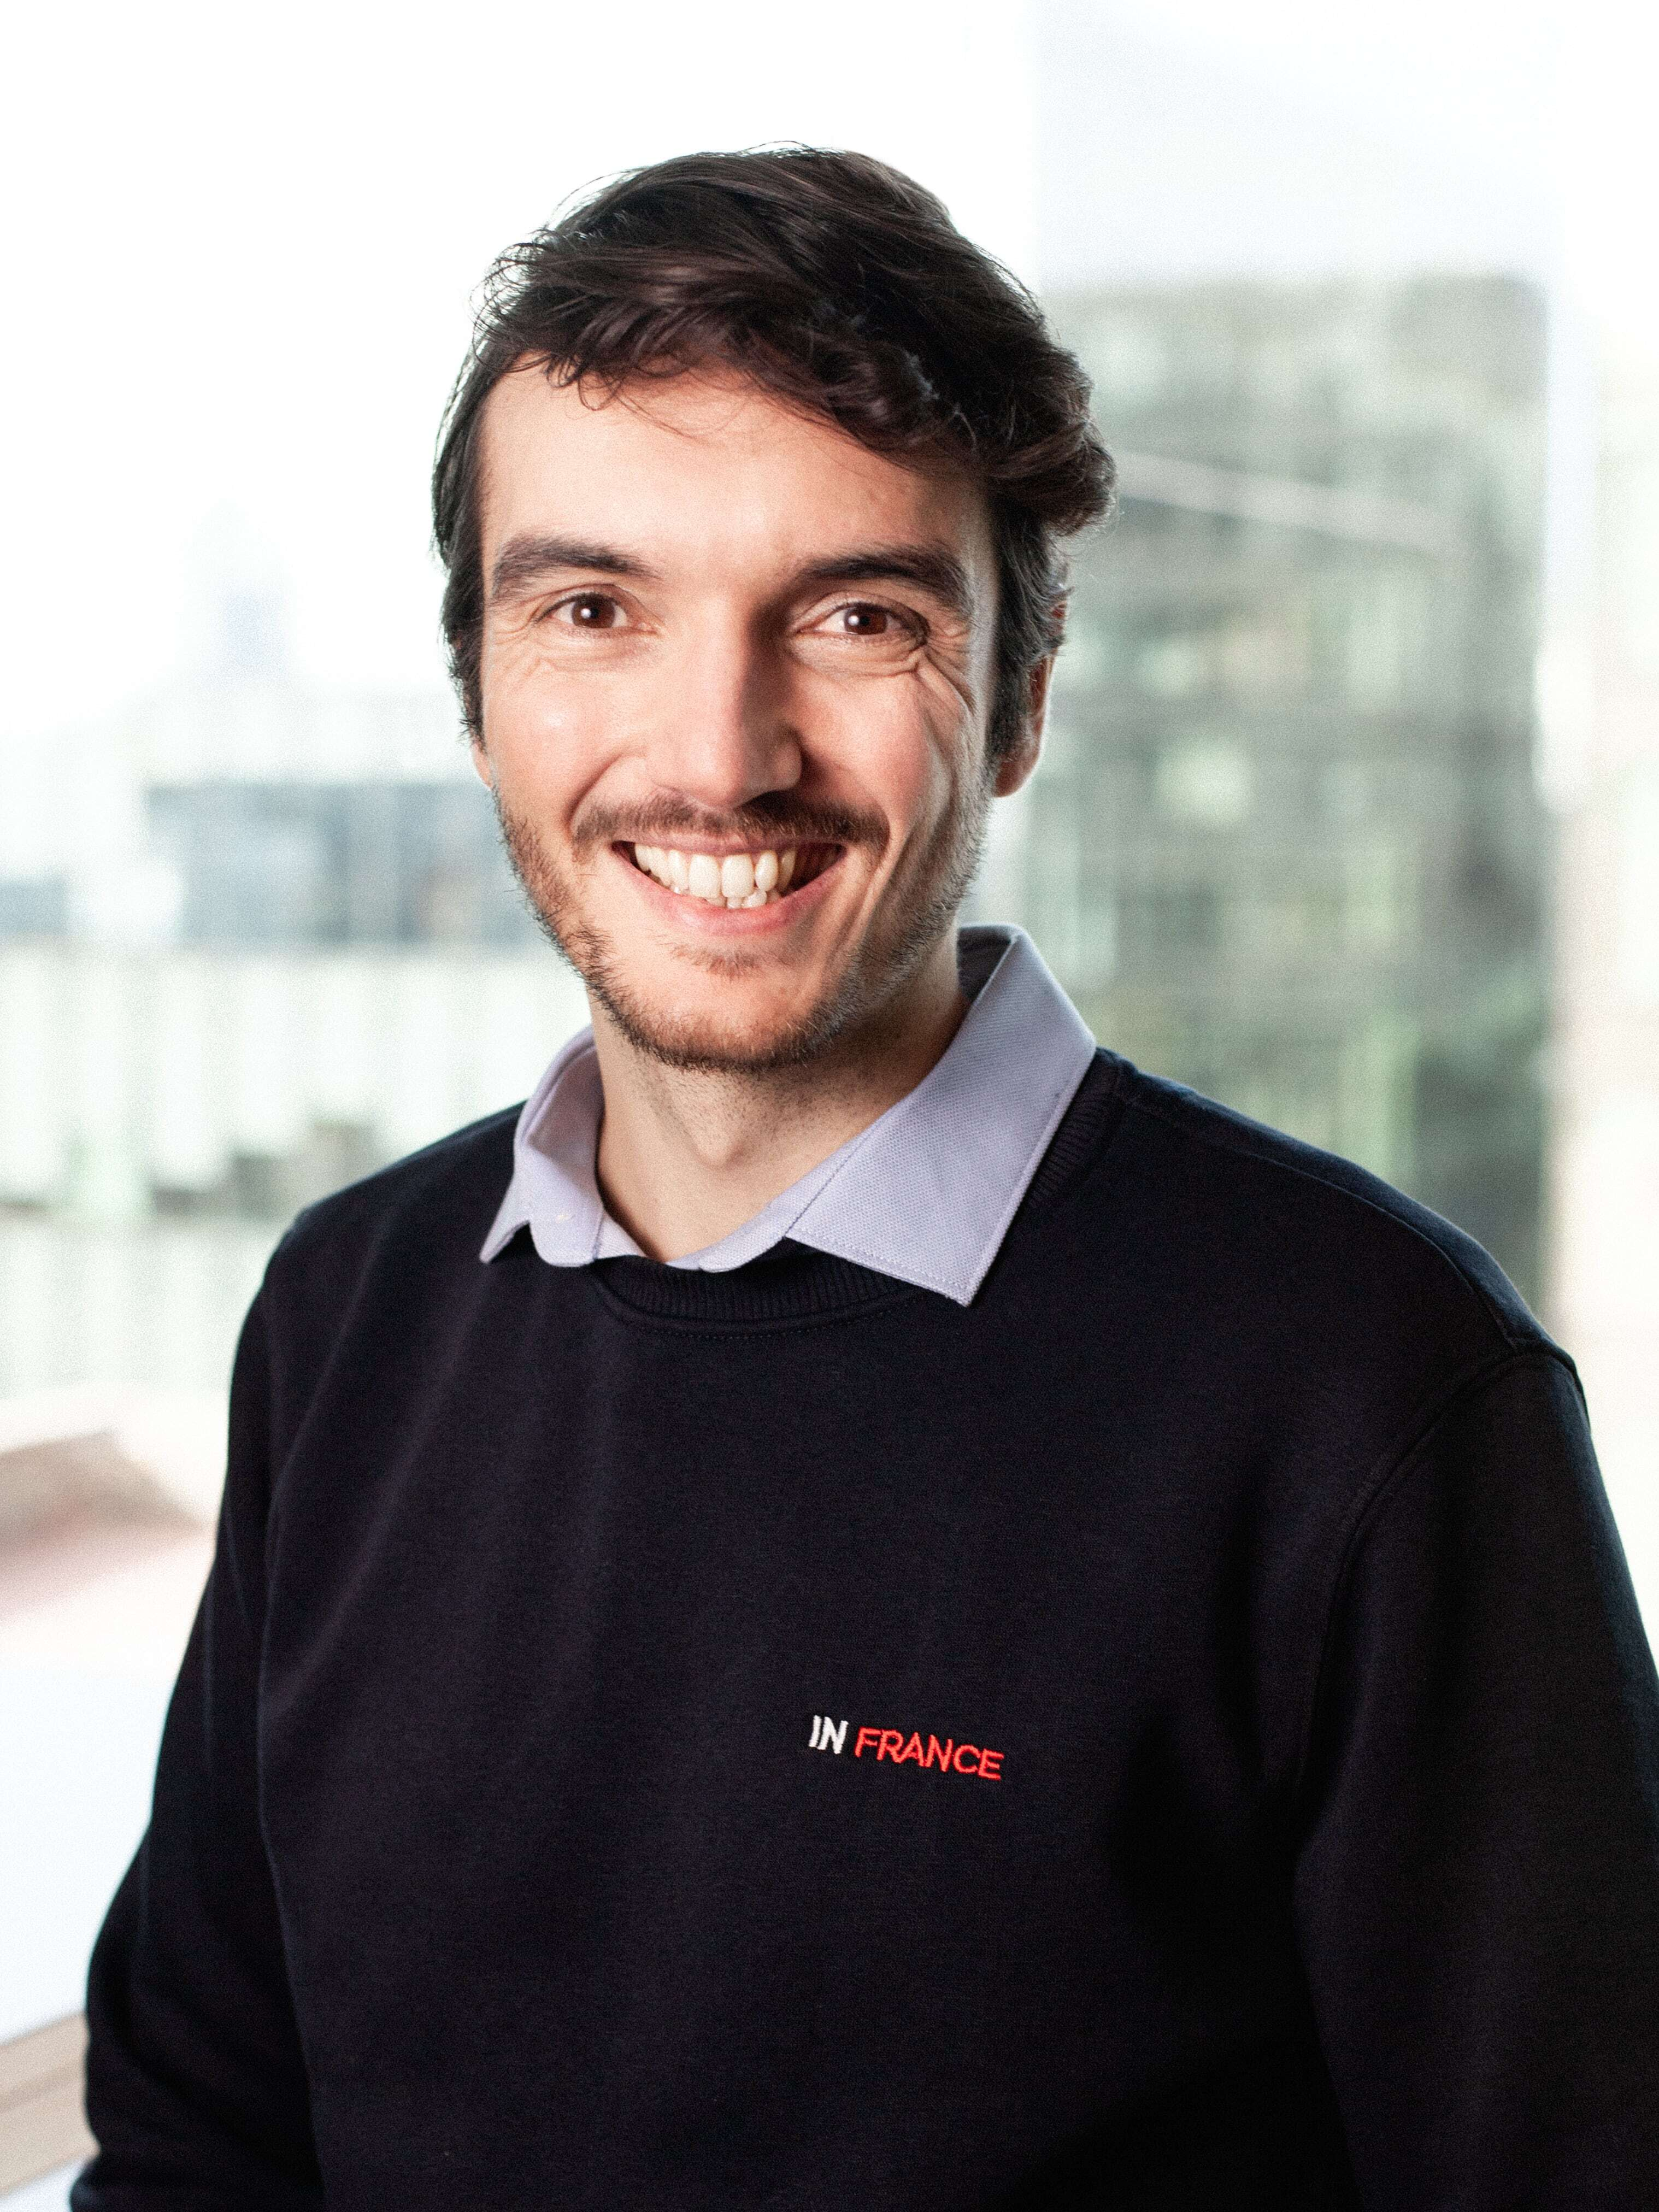
\includegraphics[width=5cm]{image/trombine-christophe}
        \end{columns}
    \end{frame}


    \section{Licence CC}\label{sec:licence}

    \begin{frame}{Licence}{Licence Creative Commons}
        Support de cours sous licence Creative Commons BY-NC-ND~.
        \bigbreak
        Vous pouvez donc, partager, copier, distribuer le document.
        \bigbreak
        Attribution requise à PapIT SASU - Pas d’utilisation commerciale - Pas de modification
        \bigbreak
        \centering
        
\includegraphics[width=5cm]{image/by-nc-nd-logo}
    \end{frame}


\end{document}
